\documentclass[pdflatex,sn-mathphys-num]{sn-jnl}

\usepackage{graphicx}
\usepackage{multirow}
\usepackage{amsmath,amssymb,amsfonts}
\usepackage{amsthm}
\usepackage{mathrsfs}
\usepackage[title]{appendix}
\usepackage{xcolor}
\usepackage{textcomp}
\usepackage{manyfoot}
\usepackage{booktabs}
\usepackage{algorithm}
\usepackage{algorithmicx}
\usepackage{algpseudocode}
\usepackage{listings}
\usepackage{tikz}
\usetikzlibrary{arrows.meta,positioning}

\theoremstyle{thmstyleone}
\newtheorem{theorem}{Theorem}
\newtheorem{proposition}[theorem]{Proposition}

\theoremstyle{thmstyletwo}
\newtheorem{example}{Example}
\newtheorem{remark}{Remark}

\theoremstyle{thmstylethree}
\newtheorem{definition}{Definition}

\raggedbottom
\linespread{0.97}

\begin{document}

\title[QAOA for Social Network Community Detection]{A Scalable Hybrid Quantum-Classical QAOA Framework for Max-Cut-Based Community Detection in Large-Scale Social Networks}

\author*[1]{\fnm{Rohit} \sur{Rao}}\email{rohitrr23.comp@coeptech.ac.in}

\author[1]{\fnm{Om} \sur{Shingare}}

\author[1]{\fnm{Viraj} \sur{Nalbalwar}}

\author[1]{\fnm{Shreesh} \sur{Kolhatkar}}

\author[1]{\fnm{Mukta} \sur{Nivelkar}}

\author[1]{\fnm{Sunil} \sur{Bhirud}}

\affil*[1]{\orgdiv{Department of Computer Science \& Engineering}, \orgname{COEP Technological University}, \orgaddress{\city{Pune}, \state{Maharashtra}, \postcode{411005}, \country{India}}}

\abstract{
Community detection in social networks uses surrogate objectives such as modularity, whereas the Maximum Cut (Max-Cut) formulation maximises interaction weight crossing a two-way partition but is NP-hard. This study develops a hybrid quantum-classical framework that encodes weighted Max-Cut as an Ising Hamiltonian, solves it with the Quantum Approximate Optimisation Algorithm (QAOA) whose angles are tuned by the COBYLA optimiser, and extends it beyond circuit qubit limits through a block-coordinate decomposition using a fixed number of qubits per subproblem. Qiskit 2.6.0 and Qiskit-Aer were used to evaluate a 16-node, 26-edge weighted graph; enumeration verified its optimum cut of 44. At depths $p=1$ to $3$ with 2\,048 shots, sampling returned an optimal cut in every case, and trained circuits assigned 100 to 300 times more probability to optimal cuts than uniform guessing, with an expected-cut ratio of 0.80 to 0.85. Greedy local search and Goemans--Williamson rounding also reached the optimum, so no quantum advantage is claimed. A simulated calibration-based IBM Sherbrooke noise model lowered the expected-cut ratio to 0.74 at $p=1$ and 0.68 at $p=2$. The block-coordinate variant, using 12-qubit subproblems, processed synthetic scale-free graphs of up to 20\,000 nodes with a fixed 12-qubit block size and matched or exceeded a greedy baseline up to 3\,000 nodes. Costs at larger scales are extrapolations of simulated block time. The experimental findings delimit shallow QAOA on small instances and demonstrate an architecture through which fixed-size quantum subproblems can serve large graphs.
}

\keywords{Quantum Approximate Optimisation Algorithm, Max-Cut, Community Detection, Variational Quantum Algorithms, NISQ, Block Decomposition, Hybrid Quantum-Classical Optimisation}

\maketitle

%%==========================================================================
\section{Introduction}\label{sec:intro}
%%==========================================================================

Online social platforms generate interaction graphs with billions of users, and the communities that emerge within them, groups bound by shared interests, geography or behaviour, underpin recommendation, misinformation containment and organisational analysis~\cite{fortunato2010community}. Community detection has consequently been studied through quality functions, most prominently modularity~\cite{newman2004finding}, which the Louvain algorithm optimises at near-linear cost on very large networks~\cite{blondel2008fast}. Such methods optimise a surrogate for community structure, however, and do not quantify how strongly two communities interact across their boundary, which is the quantity that governs information flow and influence between them.

The Maximum Cut (Max-Cut) problem expresses this interaction directly: a weighted graph is divided into two sets so that the total weight of edges joining the sets is as large as possible. Its output is therefore an interaction-maximising two-way partition, not conventional assortative community recovery, which seeks dense connections within groups. Max-Cut is NP-hard~\cite{karp1972reducibility}, so the $2^{n}$ possible partitions of an $n$-node graph cannot be enumerated beyond small $n$. The best polynomial-time guarantee is the $0.878$ ratio of the semidefinite programming relaxation of Goemans and Williamson~\cite{goemans1995improved}, which cannot be improved by any polynomial-time algorithm if the Unique Games Conjecture holds~\cite{khot2007optimal}. Classical practice therefore relies on heuristics whose solution quality on weighted social graphs is not guaranteed.

Quantum computing offers a computationally different route. Noisy intermediate-scale quantum (NISQ) processors are limited in qubit count and gate fidelity~\cite{preskill2018quantum}, which motivated variational algorithms in which a shallow parameterised circuit is tuned by a classical optimiser~\cite{peruzzo2014variational,cerezo2021variational}. The Quantum Approximate Optimisation Algorithm (QAOA)~\cite{farhi2014quantum} applies this principle to combinatorial problems such as Max-Cut. It has been executed on superconducting hardware for graphs of up to 23 qubits~\cite{harrigan2021quantum}, and its performance and operating mechanism have been analysed as the number of layers grows~\cite{zhou2020quantum}. Two obstacles temper this progress. Gradients of variational cost functions can vanish exponentially with system size~\cite{mcclean2018barren}, and low-depth QAOA faces structural limits that allow classical algorithms to outperform it on some graph families~\cite{bravyi2020obstacles}.

Evidence for QAOA is nevertheless drawn predominantly from regular or random graphs, whereas social interaction graphs are weighted and irregular. Reported success is frequently the best bitstring among the measured samples, which can be reached by uniform sampling on small graphs and therefore says little about the quantum state. Because one qubit is needed per node and exact classical simulation doubles in memory with every added qubit, a single circuit cannot represent a network of realistic size, and the route from a validated small instance to a large network is rarely specified.

The problem addressed is therefore twofold: to establish, against the exact optimum and classical baselines and under hardware noise, how well shallow QAOA partitions a weighted social graph, and to determine whether a decomposition that fixes the number of qubits per subproblem can extend the method to graphs far beyond one circuit. The work contributes an end-to-end formulation of weighted Max-Cut as an Ising Hamiltonian solved by QAOA with a verified simulator, an evaluation that separates state quality from sampling luck and compares against Louvain, spectral bisection, greedy search and Goemans--Williamson rounding, and a block-coordinate hybrid solver that is measured on graphs of up to 20\,000 nodes.

The remainder is organised as follows. Section~\ref{sec:lit} reviews literature on Max-Cut, community detection and QAOA. Section~\ref{sec:model} presents the proposed model, including the Ising encoding, QAOA circuit, classical optimiser, block decomposition and execution backends. Section~\ref{sec:results} gives the experimental setup, evaluation metrics and results on solution quality, noise and scalability. Section~\ref{sec:conclusion} summarises the findings and future directions.

%%==========================================================================
\section{Literature Review}\label{sec:lit}
%%==========================================================================

The complexity of Max-Cut was settled by Karp, who included it among the original NP-complete problems~\cite{karp1972reducibility}. Goemans and Williamson obtained a $0.878$-approximation by relaxing the problem to a semidefinite program and rounding with a random hyperplane~\cite{goemans1995improved}, and Khot et al.\ showed that this ratio is optimal for polynomial-time algorithms under the Unique Games Conjecture~\cite{khot2007optimal}. The semidefinite relaxation remains the reference for solution quality on weighted graphs but scales poorly, which is why greedy and spectral heuristics dominate large-scale practice.

Community detection has followed a separate line. Newman and Girvan introduced modularity as an objective~\cite{newman2004finding}, Blondel et al.\ made its optimisation practical on networks with millions of nodes~\cite{blondel2008fast}, and Fortunato surveyed spectral, statistical and information-theoretic alternatives~\cite{fortunato2010community}. Graph neural networks extend these methods and operate on spectral representations of graphs~\cite{bruna2013spectral}, but they depend on training data and offer no optimality guarantee. A property common to all of these methods is that they optimise modularity, conductance or label agreement rather than the cut weight, so the partitions they return need not maximise cross-community interaction.

Mapping Max-Cut to quantum hardware relies on its Ising formulation, in which binary variables become spins and the objective becomes a sum of two-body terms; Lucas catalogued such formulations for many NP problems~\cite{lucas2014ising}. QAOA, proposed by Farhi et al., prepares the state generated by alternating the Ising cost operator and a transverse-field mixer~\cite{farhi2014quantum}. Zhou et al.\ showed that performance improves with the number of layers and explained the mechanism through the structure of optimal parameters~\cite{zhou2020quantum}, and Crooks reported numerical Max-Cut results for increasing depth~\cite{crooks2018performance}. Harrigan et al.\ executed QAOA for graphs of up to 23 qubits on a superconducting processor and reported that hardware noise limited the benefit of additional layers~\cite{harrigan2021quantum}. Bravyi et al.\ proved that low-depth QAOA is limited by symmetry protection on some graph families, which cautions against assuming an advantage at small depth~\cite{bravyi2020obstacles}.

Training the angles is itself a difficulty. McClean et al.\ showed that cost gradients vanish exponentially with qubit number for sufficiently expressive circuits~\cite{mcclean2018barren}, so shallow circuits, small instances and derivative-free optimisers are the practical regime, and Amaro et al.\ proposed filtering operators that accelerate convergence of variational algorithms on combinatorial problems~\cite{amaro2022filtering}. Qiskit provides statevector and noisy shot-based simulation together with access to IBM hardware~\cite{qiskit2023}, while PennyLane offers differentiable hybrid computation with comparable circuit support~\cite{bergholm2018pennylane}.

The reviewed work leaves three gaps. Weighted, irregular social-network graphs are rarely used as QAOA benchmarks. Reported quality is seldom separated into the properties of the prepared state and the outcome of finite sampling, and the comparison with exact optima and strong classical heuristics under hardware noise is incomplete. Finally, methods for carrying a validated small-instance circuit to graphs far larger than the available qubit count are not specified. The framework developed in the following sections is designed to close these gaps.

%%==========================================================================
\section{Proposed Model}\label{sec:model}
%%==========================================================================

\subsection{System Methodology Overview}\label{sec:overview}

Figure~\ref{fig:architecture} shows the architecture of the framework. A weighted graph is read into a NetworkX graph object~\cite{hagberg2008exploring}. For graphs that exceed the qubit budget, a block-decomposition stage (Section~\ref{sec:blocks}) selects connected blocks and converts edges to the remaining nodes into fixed fields, while a small graph forms a single block. A Hamiltonian encoder produces the Ising cost operator, which feeds the QAOA circuit builder. The circuit builder and the classical optimiser exchange the measured expected cut and updated variational angles until convergence, and the best measured bitstring is then decoded into communities. Circuits run on the Qiskit-Aer simulator, with or without a device noise model, and the same circuit can be submitted to IBM hardware.

\begin{figure}[h]
\centering
\resizebox{\textwidth}{!}{%
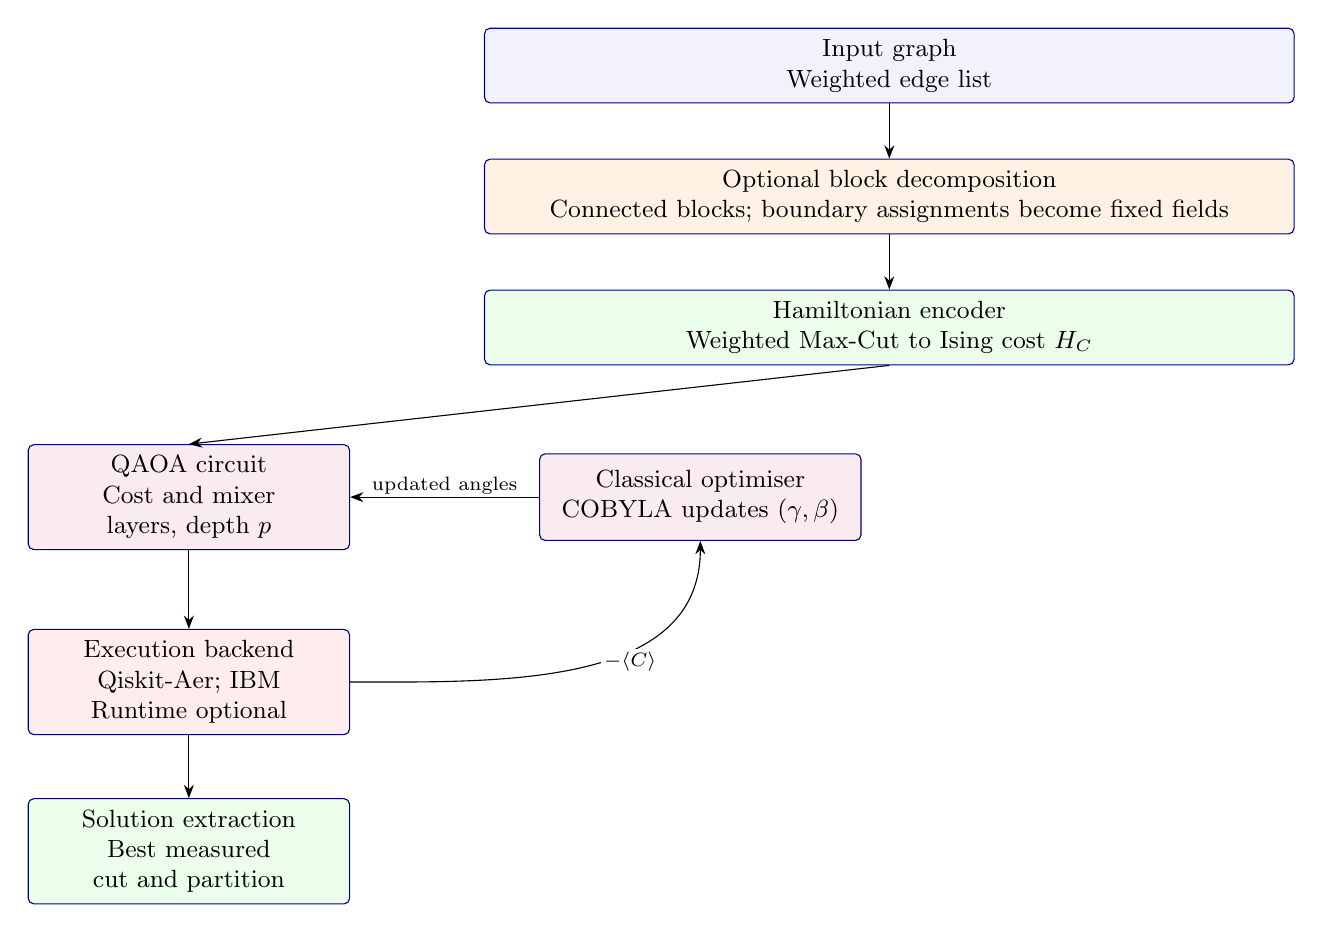
\begin{tikzpicture}[
  >=Stealth,
  font=\small,
  wide/.style={draw=blue!55!black, fill=blue!5, rounded corners=2pt, align=center, text width=10cm, minimum height=9mm, inner sep=4pt},
  stage/.style={draw=blue!55!black, rounded corners=2pt, align=center, text width=3.8cm, minimum height=11mm, inner sep=4pt}
]
\node[wide] (input) {Input graph\\Weighted edge list};
\node[wide, below=7mm of input, fill=orange!10] (blocks) {Optional block decomposition\\Connected blocks; boundary assignments become fixed fields};
\node[wide, below=7mm of blocks, fill=green!8] (ham) {Hamiltonian encoder\\Weighted Max-Cut to Ising cost $H_C$};
\node[stage, below left=10mm and 17mm of ham, fill=purple!8] (circuit) {QAOA circuit\\Cost and mixer layers, depth $p$};
\node[stage, right=24mm of circuit, fill=purple!8] (optimiser) {Classical optimiser\\COBYLA updates $(\gamma,\beta)$};
\node[stage, below=10mm of circuit, fill=red!7] (backend) {Execution backend\\Qiskit-Aer; IBM Runtime optional};
\node[stage, below=8mm of backend, fill=green!8] (solution) {Solution extraction\\Best measured cut and partition};
\draw[->] (input) -- (blocks);
\draw[->] (blocks) -- (ham);
\draw[->] (ham.south) -- (circuit.north);
\draw[->] (circuit.south) -- (backend.north);
\draw[->] (backend.south) -- (solution.north);
\draw[->] (backend.east) to[out=0,in=-90] node[pos=0.55,right,fill=white,inner sep=1pt,font=\scriptsize] {$-\langle C\rangle$} (optimiser.south);
\draw[->] (optimiser.west) -- node[above,fill=white,inner sep=1pt,font=\scriptsize] {updated angles} (circuit.east);
\end{tikzpicture}
}
\caption{Architecture of the block-QAOA workflow and its optimiser feedback.}
\label{fig:architecture}
\end{figure}

Figure~\ref{fig:workflow} summarises the pipeline for one block as four stages: graph ingestion into a weighted edge list, construction of the parameterised circuit with $p$ layers, optimisation of the angles by repeated circuit evaluation, and extraction of the partition from the optimised circuit.

\begin{figure}[h]
\centering
\resizebox{\textwidth}{!}{%
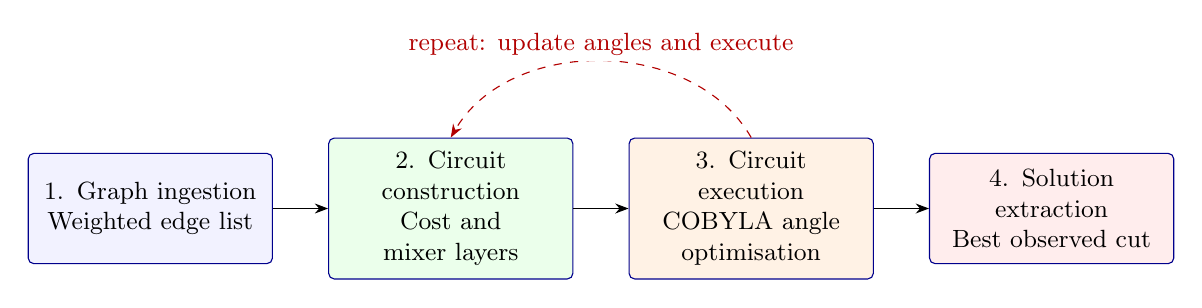
\begin{tikzpicture}[
  >=Stealth,
  font=\small,
  stage/.style={draw=blue!55!black, rounded corners=2pt, align=center, text width=2.75cm, minimum height=14mm, inner sep=5pt}
]
\node[stage, fill=blue!5] (graph) {1. Graph ingestion\\Weighted edge list};
\node[stage, fill=green!8, right=7mm of graph] (build) {2. Circuit construction\\Cost and mixer layers};
\node[stage, fill=orange!10, right=7mm of build] (optimise) {3. Circuit execution\\COBYLA angle optimisation};
\node[stage, fill=red!7, right=7mm of optimise] (extract) {4. Solution extraction\\Best observed cut};
\draw[->] (graph) -- (build);
\draw[->] (build) -- (optimise);
\draw[->] (optimise) -- (extract);
\draw[->, dashed, red!70!black] (optimise.north) to[out=120,in=60] node[above,fill=white,inner sep=2pt] {repeat: update angles and execute} (build.north);
\end{tikzpicture}%
}
\caption{Four-stage QAOA workflow with a repeated optimisation loop.}
\label{fig:workflow}
\end{figure}

\subsection{Problem Formulation and Ising Encoding}\label{sec:formulation}

Let $G=(V,E,w)$ be a weighted undirected graph with $n=|V|$ nodes, $m=|E|$ edges and weights $w_{ij}>0$ that quantify interaction strength. Nodes receive indices $0,\ldots,n-1$ that coincide with qubit labels. A partition is a vector $\mathbf{z}\in\{0,1\}^n$, with $z_i=0$ placing user $i$ in Group~A and $z_i=1$ in Group~B, and its cut value is
\begin{equation}
  C(\mathbf{z}) = \sum_{(i,j)\in E} w_{ij}\,\mathbf{1}[z_i\neq z_j],
  \label{eq:maxcut}
\end{equation}
where $\mathbf{1}[\cdot]$ is the indicator function. The community partition is $\mathbf{z}^{*}=\arg\max_{\mathbf{z}} C(\mathbf{z})$.

Substituting $z_i=(1-Z_i)/2$, with $Z_i$ the Pauli-$Z$ operator on qubit $i$, turns Eq.~\eqref{eq:maxcut} into the cost Hamiltonian
\begin{equation}
  H_C = \sum_{(i,j)\in E} \frac{w_{ij}}{2}\bigl(I - Z_iZ_j\bigr),
  \label{eq:hc}
\end{equation}
which is diagonal in the computational basis with eigenvalue $C(\mathbf{z})$ on state $|\mathbf{z}\rangle$. The identity term only shifts the spectrum, so maximising $\langle H_C\rangle$ is equivalent to maximising
\begin{equation}
  H_C^{\mathrm{eff}} = -\frac{1}{2}\sum_{(i,j)\in E} w_{ij}Z_iZ_j.
  \label{eq:hc_eff}
\end{equation}
Both $\mathbf{z}$ and its bitwise complement have the same cut value, so optimal partitions occur in pairs.

\subsection{QAOA Circuit Construction}\label{sec:circuit}

QAOA prepares the $p$-layer state
\begin{equation}
  |\psi(\boldsymbol{\gamma},\boldsymbol{\beta})\rangle = U_B(\beta_p)U_C(\gamma_p)\cdots U_B(\beta_1)U_C(\gamma_1)|{+}\rangle^{\otimes n},
  \label{eq:qaoa_state}
\end{equation}
where $|{+}\rangle^{\otimes n}=H^{\otimes n}|0\rangle^{\otimes n}$ is the equal superposition of all $2^n$ partitions produced by one Hadamard layer,
\begin{equation}
  |{+}\rangle^{\otimes n} = \frac{1}{\sqrt{2^n}}\sum_{\mathbf{z}\in\{0,1\}^n}|\mathbf{z}\rangle .
  \label{eq:init}
\end{equation}
The cost unitary applies a phase proportional to each partition's cut value and decomposes into one two-qubit rotation per edge,
\begin{equation}
  U_C(\gamma_k) = e^{-i\gamma_k H_C} \simeq \prod_{(i,j)\in E}\mathrm{RZZ}\bigl(-\gamma_k w_{ij}\bigr),
  \qquad \mathrm{RZZ}(\theta)=e^{-i\frac{\theta}{2}Z\otimes Z},
  \label{eq:uc}
\end{equation}
where $\simeq$ denotes equality up to a global phase. The mixer unitary, generated by $H_B=\sum_i X_i$, is a product of single-qubit rotations,
\begin{equation}
  U_B(\beta_k) = e^{-i\beta_k H_B} = \prod_{i=0}^{n-1} R_X(2\beta_k).
  \label{eq:ub}
\end{equation}
Each $\mathrm{RZZ}$ compiles into two CNOT gates, so a depth-$p$ circuit contains $2pm$ CNOT gates and $pn$ $R_X$ gates, linear in the number of edges. The $2p$ angles $\boldsymbol{\gamma}=(\gamma_1,\ldots,\gamma_p)$ and $\boldsymbol{\beta}=(\beta_1,\ldots,\beta_p)$ are the only trainable quantities.

\subsection{Classical Parameter Optimisation}\label{sec:cobyla}

Angles are tuned by COBYLA, a derivative-free trust-region method that builds linear models of the objective from simplex vertices~\cite{powell1994direct}. A derivative-free method is used because the objective is estimated from finite shots and is therefore noisy, and because gradient estimation by the parameter-shift rule would multiply the number of circuit executions. With $c(\mathbf{z})$ the count of bitstring $\mathbf{z}$ in $S$ shots, the objective is the negative measured expected cut,
\begin{equation}
  f(\boldsymbol{\gamma},\boldsymbol{\beta}) = -\langle C\rangle = -\frac{1}{S}\sum_{\mathbf{z}} c(\mathbf{z})\,C(\mathbf{z}).
  \label{eq:cobyla_obj}
\end{equation}
Initial angles are drawn as $\gamma_k\sim\mathcal{U}[0,\pi]$ and $\beta_k\sim\mathcal{U}[0,\pi/2]$ from a seeded generator, the initial trust-region radius is $0.5$ rad, and the best of several random restarts is retained. Algorithm~\ref{alg:qaoa} lists the procedure.

\begin{algorithm}[t]
\caption{Shot-based QAOA training for weighted Max-Cut}\label{alg:qaoa}
\begin{algorithmic}[1]
\Require Graph $G=(V,E,w)$, depth $p$, shots $S$, iteration cap $T$, restarts $R$
\Ensure Partition $\mathbf{z}^*$ and cut value $C(\mathbf{z}^*)$
\State Build the parameterised circuit of Eq.~\eqref{eq:qaoa_state}
\For{$r = 1,\ldots,R$}
  \State Draw $\boldsymbol{\gamma}^{(0)}\sim\mathcal{U}[0,\pi]^{p}$, $\boldsymbol{\beta}^{(0)}\sim\mathcal{U}[0,\pi/2]^{p}$
  \State $t\leftarrow0$
  \While{$t<T$ and COBYLA has not terminated}
    \State Bind angles and execute with $S$ shots; estimate $\langle C\rangle$ from counts
    \State Update angles by minimising $f$ in Eq.~\eqref{eq:cobyla_obj}
    \State $t\leftarrow t+1$
  \EndWhile
\EndFor
\State Keep the restart with the highest final expected cut
\State Execute at the kept angles; return $\mathbf{z}^*=\arg\max_{\mathbf{z}\in\text{observed}} C(\mathbf{z})$
\end{algorithmic}
\end{algorithm}

\subsection{Solution Extraction}\label{sec:extraction}

After convergence the circuit is executed once more at the optimal angles, and the empirical probability of each outcome is $\hat P(\mathbf{z})=c(\mathbf{z})/S$. The reported partition is the observed bitstring of highest cut value,
\begin{equation}
  \mathbf{z}^{*}=\arg\max_{\mathbf{z}\in\text{observed}} C(\mathbf{z}),
  \label{eq:extract}
\end{equation}
which can differ from the most probable bitstring for finite $S$. Qiskit reports qubit~0 as the rightmost character of a bitstring, so every key is reversed before Eq.~\eqref{eq:maxcut} is evaluated; omitting this reversal evaluates the cut on a mirrored graph and gives incorrect partitions.

\subsection{Architectural Decomposition for Large Graphs}\label{sec:blocks}

A single circuit needs one qubit per node, which is unavailable for large networks. The decomposition solves one small block at a time while all other nodes keep their current assignment. Let $E[B]$ contain edges internal to block $B$, and let $\partial B$ contain edges with exactly one endpoint in $B$. For $(i,j)\in\partial B$, write $u(i,j)$ for the endpoint inside $B$ and $v(i,j)$ for the endpoint outside it. For $|B|\le k$ and fixed outside assignment $\mathbf{z}_{\bar B}$, the quantity to maximise is
\begin{equation}
  C_B(\mathbf{z}_B) = \sum_{(i,j)\in E[B]} w_{ij}\mathbf{1}[z_i\neq z_j] + \sum_{(i,j)\in\partial B} w_{ij}\mathbf{1}[z_{u(i,j)}\neq z_{v(i,j)}],
  \label{eq:blockcost}
\end{equation}
where the outside endpoint values in the second sum are fixed. The corresponding Hamiltonian gains a single-qubit field for every boundary edge,
\begin{equation}
  H_B^{\mathrm{blk}} = \sum_{(i,j)\in E[B]}\frac{w_{ij}}{2}\bigl(I-Z_iZ_j\bigr) + \sum_{(i,j)\in\partial B}\frac{w_{ij}}{2}\bigl(I-s_{v(i,j)}Z_{u(i,j)}\bigr),
  \qquad s_v = 1-2z_v,
  \label{eq:blockham}
\end{equation}
so that the cost layer adds one $R_Z(-\gamma w_{ij}s_{v(i,j)})$ rotation per boundary edge to the $\mathrm{RZZ}$ gates of Eq.~\eqref{eq:uc}. Each block uses at most $k$ qubits irrespective of $n$. A block update is accepted only if it raises Eq.~\eqref{eq:blockcost}, so the global cut is non-decreasing. Blocks are formed from randomly seeded breadth-first traversals and redrawn in every sweep; some boundary edges may become internal edges in later sweeps. Algorithm~\ref{alg:block} lists the procedure.

\begin{algorithm}[t]
\caption{Exact-training block-coordinate QAOA}\label{alg:block}
\begin{algorithmic}[1]
\Require Graph $G$, block size $k$, depth $p$, sweeps $L$, COBYLA cap $T$, update shots $S$, initial assignment $\mathbf{z}$ (random)
\Ensure Assignment $\mathbf{z}$ with non-decreasing cut
\For{$s = 1,\ldots,L$}
  \State Partition $V$ into connected blocks of at most $k$ nodes by random breadth-first traversal
  \For{each block $B$}
    \State Build $C_B$ of Eq.~\eqref{eq:blockcost} with outside nodes fixed
    \State Train one depth-$p$ QAOA start by maximising the exact statevector expectation of $C_B$
    \State Sample the trained state $S$ times
    \State Let $\mathbf{z}_B'$ be the sampled assignment with the highest $C_B$
    \If{$C_B(\mathbf{z}_B')>C_B(\mathbf{z}_B)$} \State $\mathbf{z}_B\leftarrow\mathbf{z}_B'$ \EndIf
  \EndFor
\EndFor
\State \Return $\mathbf{z}$
\end{algorithmic}
\end{algorithm}

Because block size is capped, the number of subproblems grows linearly with $n$. In this implementation their sizes vary below the cap, so per-block runtimes are not identical; blocks without shared boundary edges may be dispatched to separate devices.

\subsection{Execution Backends and Noise Handling}\label{sec:backends}

Exact statevector simulation stores $2^n$ complex amplitudes,
\begin{equation}
  M(n) = 16\cdot 2^{n}\ \text{bytes},
  \label{eq:memory}
\end{equation}
which is about 1\,MB at $n=16$ and about 68\,GB at $n=32$, so Eq.~\eqref{eq:memory} caps monolithic simulation on a workstation near 32 qubits. The NumPy statevector computes exact outcome probabilities and is verified against Qiskit's circuit simulation. In the primary experiments, finite-shot objective values are sampled from those probabilities, and restarts are ranked by their exact expected cuts; Qiskit-Aer independently executes the circuit for final sampling and noisy runs. Block-coordinate optimisation uses exact statevector expectations and samples 1\,024 outcomes only when selecting a proposed update. On physical NISQ devices, two-qubit errors compound as entangling-gate counts grow, as observed in superconducting QAOA experiments~\cite{harrigan2021quantum}. Zero-noise extrapolation, which recovers an ideal value from runs at amplified noise levels~\cite{temme2017error}, readout-error calibration and transpilation to the device topology are applicable mitigation steps. Logical qubits protected by surface codes~\cite{fowler2012surface} would reduce noise but require orders of magnitude more physical qubits, and are therefore a long-term target.

%%==========================================================================
\section{Results and Discussion}\label{sec:results}
%%==========================================================================

\subsection{Experimental Setup}\label{sec:setup}

The primary instance is a hand-constructed 16-node, 26-edge weighted graph with integer weights in $\{1,2,3\}$, total weight 52 and node degrees between 2 and 5. Because $2^{16}=65\,536$ partitions can be scored at once, the exact optimum was obtained by enumeration in about 8\,ms: the maximum cut is 44, attained by 6 bit patterns forming 3 partitions and their complements. A uniformly random partition cuts 26 on average, which is 59.1\% of the optimum. Scalability experiments use Barab\'asi--Albert graphs with three edges per new node and integer weights drawn from $\{1,2,3\}$. Table~\ref{tab:config} lists the configuration. The NumPy simulator reproduces the measurement probabilities of the Qiskit circuit to within $3\times10^{-18}$, so the two are interchangeable.

\begin{table}[h]
\caption{Simulation, noise-model and block-solver settings.}\label{tab:config}
\begin{tabular}{@{}p{0.28\textwidth}p{0.62\textwidth}@{}}
\toprule
Parameter & Value \\
\midrule
Primary network & 16 nodes, 26 edges, weights in $\{1,2,3\}$, total weight 52 \\
Circuit depth $p$ & 1, 2, 3 \\
Primary QAOA shots $S$ per objective evaluation & 2\,048 \\
COBYLA iteration cap, initial radius & 300, 0.5 rad \\
Initial angles & $\gamma\sim\mathcal{U}[0,\pi]$, $\beta\sim\mathcal{U}[0,\pi/2]$, best of 5 restarts, seed 42 \\
Simulators & NumPy statevector (training), Qiskit-Aer (sampling, noise) \\
Noise model & Simulated FakeSherbrooke calibration (IBM Eagle) \\
Block-coordinate solver & $k=12$, $p=2$, 3 sweeps; exact training, 1\,024 update samples, 60 iterations (40 at 20\,000 nodes) \\
Software & Python 3.14.8, Qiskit 2.6.0, Qiskit-Aer 0.18.0 \\
\botrule
\end{tabular}
\end{table}

Four classical baselines run on the same graphs. Spectral bisection thresholds the dominant eigenvector of the weighted Laplacian. Greedy 1-flip repeatedly moves single nodes that raise the cut, from 10 random starts on the primary graph and 3 on the scalability graphs. The Goemans--Williamson baseline solves the semidefinite relaxation and rounds with 20 random hyperplanes. Louvain communities are merged into two groups by exhaustive search over community colourings.

\subsection{Evaluation Metrics}\label{sec:metrics}

The best bitstring among $S$ samples is a weak indicator on a 16-qubit instance, because 2\,048 uniformly random partitions already contain an optimum in 14.2\% of trials and have a mean best cut of 42.4. Three quantities are therefore reported. At the selected angles, exact statevector probabilities $P_{\theta}(\mathbf{z})$ measure the quality of the whole QAOA distribution; the primary COBYLA objective is separately estimated from finite-shot counts. The expected-cut ratio is
\begin{equation}
  \rho = \frac{\langle C\rangle_{\theta}}{C_{\max}}, \qquad \langle C\rangle_{\theta}=\sum_{\mathbf{z}}P_{\theta}(\mathbf{z})\,C(\mathbf{z}),
  \label{eq:rho}
\end{equation}
where $C_{\max}$ is the exact optimum. The optimal-sampling probability is
\begin{equation}
  P_{\mathrm{opt}} = \sum_{\mathbf{z}:\,C(\mathbf{z})=C_{\max}}P_{\theta}(\mathbf{z}),
  \label{eq:popt}
\end{equation}
which equals $6/2^{16}\approx9\times10^{-5}$ for the uniform distribution, so the enrichment $P_{\mathrm{opt}}/(6/2^{16})$ measures how much probability the circuit concentrates on optimal cuts. The third quantity is the best cut among the $S$ measured shots, which is what Eq.~\eqref{eq:extract} returns. Uniform random sampling of $S$ partitions controls for this best-of-shots metric.

\subsection{Performance of the Trained Circuits}\label{sec:training}

Table~\ref{tab:training} reports the best of five restarts at each depth. COBYLA stopped after 36 to 67 evaluations, far below the cap of 300. Figure~\ref{fig:convergence} shows the measured expected cut over the evaluations of the best restart. At $p=2$ the optimal angles were $\boldsymbol{\gamma}=(2.66,3.35)$ and $\boldsymbol{\beta}=(0.03,1.22)$.

\begin{table}[h]
\caption{Five-restart primary QAOA results; restarts ranked by exact expected cut.}\label{tab:training}
\begin{tabular}{@{}lccccc@{}}
\toprule
Depth & Selected-restart evaluations & $\rho$ & $P_{\mathrm{opt}}$ & Enrichment & Best of $S$ shots \\
\midrule
$p=1$ & 36 & 0.799 & 1.07\% & 117$\times$ & 44 \\
$p=2$ & 53 & 0.796 & 1.00\% & 109$\times$ & 44 \\
$p=3$ & 67 & 0.847 & 2.80\% & 305$\times$ & 44 \\
\botrule
\end{tabular}
\end{table}

\begin{figure}[h]
\centering
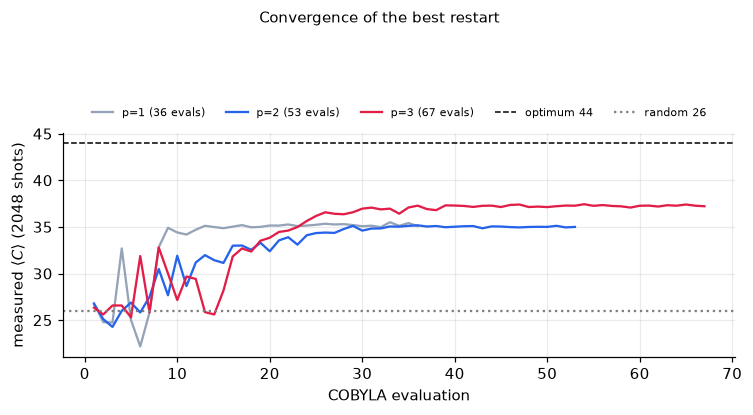
\includegraphics[width=0.6\textwidth]{fig_convergence.png}
\caption{Shot-estimated COBYLA objectives for the selected restart at each depth.}
\label{fig:convergence}
\end{figure}

A single trained circuit depends on the random start. Over 10 independent seeds with one restart each, $\rho$ was $0.704\pm0.100$ at $p=1$, $0.710\pm0.101$ at $p=2$ and $0.723\pm0.087$ at $p=3$, and the best of 2\,048 shots was at least 41 in every run, with mean 43.2 to 43.6. The differences between depths are smaller than the seed-to-seed spread, so no statistically supported gain from increasing $p$ is established for this instance with the present optimiser and budget.

\subsection{Partition and Comparison with Classical Methods}\label{sec:comparison}

Sampling the trained $p=2$ circuit on Qiskit-Aer returned optimal partitions of cut weight 44. The plotted sample, bitstring \texttt{0110010110001110}, assigns Rohit, Dave, Eve, Grace, Jack, Karen, Leo and Peter to Group~A and Bob, Carol, Frank, Henry, Isla, Mia, Nathan and Olivia to Group~B, with 20 of the 26 edges crossing the cut (Fig.~\ref{fig:results_panel}).

\begin{figure}[h]
\centering
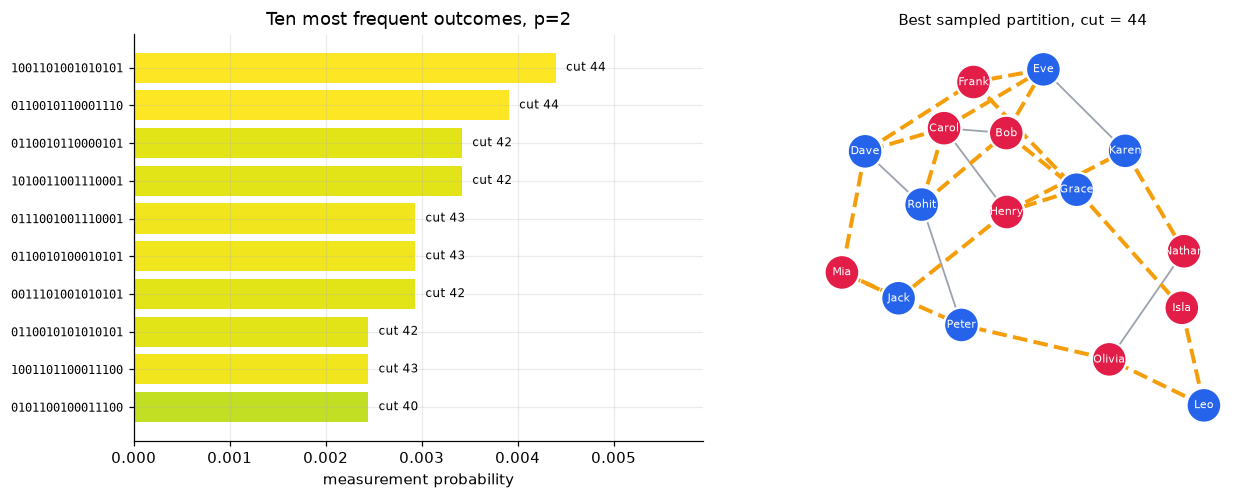
\includegraphics[width=0.95\textwidth]{fig_probabilities_partition.png}
\caption{Ten frequent $p=2$ outcomes and one optimal sample; node colors mark groups, dashed edges the cut.}
\label{fig:results_panel}
\end{figure}

Table~\ref{tab:comparison} compares all methods on the same graph. Louvain scores low by construction, because maximising modularity favours few edges between communities and therefore opposes Max-Cut.

\begin{table}[h]
\caption{Classical and QAOA cut values on the 16-node network.}\label{tab:comparison}
\begin{tabular*}{\textwidth}{@{\extracolsep\fill}lcc}
\toprule
Method & Cut value & Share of optimum (\%) \\
\midrule
Random partition (mean) & 26.0 & 59.1 \\
Louvain, communities merged into two groups & 10.0 & 22.7 \\
Spectral bisection & 39.0 & 88.6 \\
Goemans--Williamson, mean of 20 roundings$^{\text{(a)}}$ & 41.95 & 95.3 \\
Random sampling, best of 2\,048 (mean of 500 trials) & 42.4 & 96.4 \\
QAOA expected cut, $p=2$ & 35.0 & 79.6 \\
QAOA best of 2\,048 shots, $p=1,2,3$ & 44.0 & 100.0 \\
Goemans--Williamson, best of 20 roundings & 44.0 & 100.0 \\
Greedy 1-flip, 10 restarts & 44.0 & 100.0 \\
Brute-force optimum & 44.0 & 100.0 \\
\botrule
\end{tabular*}
\footnotetext{(a) The semidefinite upper bound is 45.78.}
\end{table}

\subsection{Effect of Hardware Noise}\label{sec:noise}

Angles trained under ideal simulation were executed in Aer using the calibration-derived FakeSherbrooke noise model after transpilation to its native gates. The expected-cut ratio fell from 0.799 to 0.743 at $p=1$, where the transpiled circuit has 127 two-qubit gates and depth 322, and from 0.796 to 0.682 at $p=2$, with 251 two-qubit gates and depth 642. The deeper circuit therefore moves further towards the random level of 0.591, while the best sampled cut remained 44 in both cases.

\subsection{Scalability of the Block-Coordinate Solver}\label{sec:scalability}

Table~\ref{tab:scalability} reports the block-coordinate solver of Algorithm~\ref{alg:block} on scale-free graphs. At 100 nodes the Goemans--Williamson best rounding reached 468 against a semidefinite upper bound of 500.1. The solver was ahead of the greedy baseline by 0.6 to 2.7\% at 300 to 3\,000 nodes, although that baseline used only 3 restarts. A single sweep over a graph of 20\,000 nodes and 59\,991 edges solved 2\,187 blocks in 69\,s and reached 71.4\% of the total weight, against 74.6\% for one greedy run, so additional sweeps are needed at that size (Fig.~\ref{fig:block_scaling}, right). The measured mean was about 32\,ms per block in the 20\,000-node run, and the number of blocks was about 0.109 per node because breadth-first blocks averaged fewer than 12 nodes. Extrapolating this simulated cost gives about 57.6\,min for one sweep over $10^{6}$ nodes and about 4.8\,h for $5\times10^{6}$ nodes on a single core, or about 3 and 17 seconds with 1\,000 ideal parallel workers. These extrapolations apply to classical simulation of 12-qubit blocks; quantum devices would add queueing, shot and mitigation overhead.

\begin{table}[h]
\caption{Three-sweep block-QAOA and classical baselines on synthetic graphs.}\label{tab:scalability}
\begin{tabular}{@{}rrrrrrr@{}}
\toprule
Nodes & Total weight & Random & Spectral & Greedy 1-flip & Block-QAOA & Time (s) \\
\midrule
100 & 606 & 303 & 394 & 457 & 464 & 1.9 \\
300 & 1\,776 & 888 & 1\,153 & 1\,329 & 1\,365 & 5.2 \\
1\,000 & 5\,930 & 2\,965 & 3\,855 & 4\,462 & 4\,488 & 15.5 \\
3\,000 & 18\,141 & 9\,071 & 12\,235 & 13\,562 & 13\,811 & 48.3 \\
\botrule
\end{tabular}
\end{table}

\begin{figure}[h]
\centering
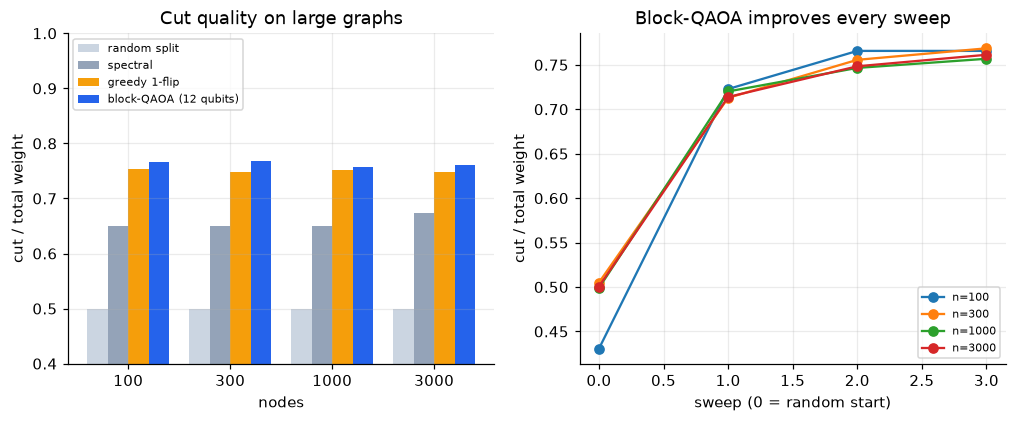
\includegraphics[width=0.95\textwidth]{fig_block_qaoa_scaling.png}
\caption{Cut ratios for four methods and block-QAOA improvement over three sweeps.}
\label{fig:block_scaling}
\end{figure}

\subsection{Discussion}\label{sec:discussion}

The experiments show that QAOA reliably prepares states that favour good cuts, with $P_{\mathrm{opt}}$ between 100 and 300 times the uniform value and $\rho$ between 0.80 and 0.85, yet this does not translate into an advantage on the 16-node graph. Greedy local search, Goemans--Williamson rounding and even uniform sampling match the best sampled cut of 44, and the effect of depth on $\rho$ is smaller than the variation across random starts. The best bitstring among samples is therefore an inadequate quality measure for small instances, whereas $\rho$ and $P_{\mathrm{opt}}$ expose the state itself. Noise reduces $\rho$ more at $p=2$ than at $p=1$, so on NISQ devices additional layers can be counterproductive unless error mitigation recovers the loss.

The block-coordinate solver turns the validated small circuit into a unit of a larger computation. Its maximum block size is independent of graph size and its cut does not decrease across sweeps by construction. On graphs of 300 to 3\,000 nodes it exceeded a lightly tuned greedy baseline, but it trailed a single greedy run after one sweep on 20\,000 nodes. Conclusions are bounded by the hand-built primary graph, the synthetic scale-free graphs, the absence of execution on physical hardware, and the status of figures above 20\,000 nodes as extrapolations. A quantum benefit at scale would require subproblems on hardware whose fidelity supports more than a few layers, and a comparison with classical solvers tuned to the same time budget.

%%==========================================================================
\section{Conclusion and Future Scope}\label{sec:conclusion}
%%==========================================================================

The work formulated weighted Max-Cut community detection as an Ising Hamiltonian, solved it with QAOA tuned by COBYLA, and extended it to large graphs through a block-coordinate decomposition. On a 16-node graph with a verified optimum of 44, depths one to three returned an optimal cut, and the trained circuits placed 100 to 300 times more probability on optimal partitions than uniform guessing, with expected-cut ratios of 0.80 to 0.85. Greedy search and Goemans--Williamson rounding performed equally well, so no quantum advantage follows from these results. Simulated hardware noise reduced the expected-cut ratio to 0.74 and 0.68 at depths one and two. The block-coordinate solver processed graphs of up to 20\,000 nodes with blocks capped at 12 qubits, defining an architecture through which bounded quantum subproblems can be applied to larger networks. The solver's one-sweep result at 20\,000 nodes remained below the greedy baseline, and estimates beyond this size are extrapolations rather than experiments; both limitations constrain claims about practical scale.

Four extensions follow directly. Execution on IBM hardware with zero-noise extrapolation and readout-error mitigation would replace noise-model estimates with physical measurements. Tensor-network simulation is a candidate for evaluating larger blocks, but feasible sizes must be established from entanglement and resource measurements rather than assumed. Optimisers such as SPSA could reduce evaluations per block. A statistically controlled study of depths three and four with improved optimisers would test whether the approximation ratio rises with depth, which the ten-seed experiment could not resolve. Finally, real interaction data would require preprocessing for automated accounts, repeated interactions and temporal decay, and $k$-way partitioning would extend the model to more than two communities.

%%==========================================================================
\backmatter

\section*{Acknowledgements}
The authors thank Dr.~Mukta Nivelkar (Guide) and Dr.~Sunil Bhirud (Co-Guide), Department of Computer Science \& Engineering, COEP Technological University, for their supervision, technical guidance, and support throughout this work.

%%==========================================================================

\begin{thebibliography}{99}
\footnotesize
\setlength{\itemsep}{0pt}
\setlength{\parskip}{2pt}

\bibitem{fortunato2010community}
Fortunato, S.: Community detection in graphs. Phys. Rep. \textbf{486}(3--5), 75--174 (2010)

\bibitem{newman2004finding}
Newman, M.E.J., Girvan, M.: Finding and evaluating community structure in networks. Phys. Rev. E \textbf{69}(2), 026113 (2004)

\bibitem{blondel2008fast}
Blondel, V.D., Guillaume, J.-L., Lambiotte, R., Lefebvre, E.: Fast unfolding of communities in large networks. J. Stat. Mech. Theory Exp. \textbf{2008}, 10008 (2008)

\bibitem{karp1972reducibility}
Karp, R.M.: Reducibility among combinatorial problems. In: Miller, R.E., Thatcher, J.W. (eds.) Complexity of Computer Computations, pp. 85--103. Plenum Press, New York (1972)

\bibitem{goemans1995improved}
Goemans, M.X., Williamson, D.P.: Improved approximation algorithms for maximum cut and satisfiability problems using semidefinite programming. J. ACM \textbf{42}(6), 1115--1145 (1995)

\bibitem{khot2007optimal}
Khot, S., Kindler, G., Mossel, E., O'Donnell, R.: Optimal inapproximability results for MAX-CUT and other 2-variable CSPs? SIAM J. Comput. \textbf{37}(1), 319--357 (2007)

\bibitem{preskill2018quantum}
Preskill, J.: Quantum computing in the NISQ era and beyond. Quantum \textbf{2}, 79 (2018)

\bibitem{peruzzo2014variational}
Peruzzo, A., et al.: A variational eigenvalue solver on a photonic chip. Nat. Commun. \textbf{5}, 4213 (2014)

\bibitem{cerezo2021variational}
Cerezo, M., et al.: Variational quantum algorithms. Nat. Rev. Phys. \textbf{3}, 625--644 (2021)

\bibitem{farhi2014quantum}
Farhi, E., Goldstone, J., Gutmann, S.: A quantum approximate optimization algorithm. arXiv:1411.4028 (2014)

\bibitem{harrigan2021quantum}
Harrigan, M.P., et al.: Quantum approximate optimization of non-planar graph problems on a planar superconducting processor. Nat. Phys. \textbf{17}, 332--336 (2021)

\bibitem{zhou2020quantum}
Zhou, L., Wang, S.-T., Choi, S., Pichler, H., Lukin, M.D.: Quantum approximate optimization algorithm: performance, mechanism, and implementation on near-term devices. Phys. Rev. X \textbf{10}(2), 021067 (2020)

\bibitem{mcclean2018barren}
McClean, J.R., Boixo, S., Smelyanskiy, V.N., Babbush, R., Neven, H.: Barren plateaus in quantum neural network training landscapes. Nat. Commun. \textbf{9}, 4812 (2018)

\bibitem{bravyi2020obstacles}
Bravyi, S., Kliesch, A., Koenig, R., Tang, E.: Obstacles to state preparation and variational optimization from symmetry protection. Phys. Rev. Lett. \textbf{125}, 260505 (2020)

\bibitem{bruna2013spectral}
Bruna, J., Zaremba, W., Szlam, A., LeCun, Y.: Spectral networks and locally connected networks on graphs. arXiv:1312.6203 (2013)

\bibitem{lucas2014ising}
Lucas, A.: Ising formulations of many NP problems. Front. Phys. \textbf{2}, 5 (2014)

\bibitem{crooks2018performance}
Crooks, G.E.: Performance of the quantum approximate optimization algorithm on the maximum cut problem. arXiv:1811.08419 (2018)

\bibitem{amaro2022filtering}
Amaro, D., et al.: Filtering variational quantum algorithms for combinatorial optimization. Quantum Sci. Technol. \textbf{7}, 015021 (2022)

\bibitem{qiskit2023}
Qiskit contributors: Qiskit: an open-source framework for quantum computing. Zenodo (2023)

\bibitem{bergholm2018pennylane}
Bergholm, V., et al.: PennyLane: automatic differentiation of hybrid quantum-classical computations. arXiv:1811.04968 (2018)

\bibitem{hagberg2008exploring}
Hagberg, A., Swart, P., Chult, D.S.: Exploring network structure, dynamics, and function using NetworkX. In: Proceedings of the 7th Python in Science Conference (SciPy 2008), pp. 11--15 (2008)

\bibitem{powell1994direct}
Powell, M.J.D.: A direct search optimization method that models the objective and constraint functions by linear interpolation. In: Gomez, S., Hennart, J.-P. (eds.) Advances in Optimization and Numerical Analysis, pp. 51--67. Kluwer Academic, Dordrecht (1994)

\bibitem{temme2017error}
Temme, K., Bravyi, S., Gambetta, J.M.: Error mitigation for short-depth quantum circuits. Phys. Rev. Lett. \textbf{119}, 180509 (2017)

\bibitem{fowler2012surface}
Fowler, A.G., Mariantoni, M., Martinis, J.M., Cleland, A.N.: Surface codes: towards practical large-scale quantum computation. Phys. Rev. A \textbf{86}, 032324 (2012)

\end{thebibliography}

\end{document}
